
\documentclass{article}

% Deactivate sectsty warning when loading sectsty {{{
\usepackage[immediate]{silence}
\WarningFilter[temp]{latex}{Command}
\usepackage{sectsty}
    \sectionfont{\normalfont\sffamily\bfseries\color{blue!40!black}}
    \subsectionfont{\normalfont\sffamily\bfseries\color{blue!30!black}}
\DeactivateWarningFilters[temp]
\makeatletter % disable the runtime redefinitions
\let\SS@makeulinesect\relax
\let\SS@makeulinepartchap\relax
\makeatother
% }}}

\usepackage[margin=4cm]{geometry}
    \setlength\parindent{0pt}
\usepackage{fancyhdr}
    \pagestyle{fancy}
\usepackage{fontspec}
    \setsansfont{Linux Biolinum O}
\usepackage{polyglossia}
    \setmainlanguage{english}
\usepackage{sectsty}
    \sectionfont{\normalfont\sffamily\bfseries\color{blue!40!black}}
    \subsectionfont{\normalfont\sffamily\bfseries\color{blue!30!black}}
\usepackage{amsmath}
\usepackage{amssymb}
\usepackage{siunitx}
\usepackage{float}
\usepackage{booktabs}
\usepackage{subcaption}
\usepackage{graphicx}
\usepackage{xcolor}
\usepackage{listings}
    \lstset{language=Python,
	basicstyle=\footnotesize\ttfamily,
	breaklines=true,
	framextopmargin=50pt,
	frame=bottomline,
	backgroundcolor=\color{white!86!black},
	commentstyle=\color{blue},
	keywordstyle=\color{red},
	stringstyle=\color{orange!80!black}}
\usepackage{tikz}
\usepackage{hyperref}

\title{\textsf{\color{blue!40!black}5. Übung IBN}}
\author{Maurice Donner \and Ise Glade}

\begin{document}

\maketitle
\newpage

\section*{Augabe 1}
\textbf{a.} 
In Intels \textit{System programming guide} for their 64 and IA-32 Architectures
, all the necessary information about paging can be found:
\url{https://software.intel.com/sites/default/files/managed/a4/60/325384-sdm-vol-3abcd.pdf}\\
The supported page sizes for the 4-Level-Paging used on the 64-Bit
Architecture are 4KiB, 2MiB, and 1GiB. \\

\textbf{b.}
The canonical address design ensures, that there are effectively two
halves of virtual addresses. Some systems use these memory halves to
implement a \textit{user} and a \textit{kernal space}. This feature eases
later scalability into true 64-Bit addressing, because there is still a large
unused non-canonical region in memory. Because it lies in the "center" of the
virtual address space, both the lower and upper memory half can easily be
extended by increasing/decreasing the addresses of each region, respectively.
\begin{figure}[H]
    \centering
    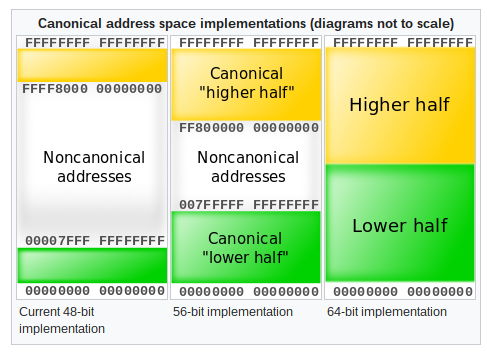
\includegraphics[width=7cm]{Canonical.png}
\end{figure}

\section*{Aufgabe 2} 
The benefit of supersections is an effectively lower amount of
required accesses. This can e.g. be benificial for operating systems,
where large regions of memory have to be loaded at all times.
This doesnt come without a trade-off though, as the chance for
internal fragmentation rises exponentially with the pagesize.

\section*{Aufgabe 4}

\section*{Aufgabe 5}

The virtual address \( \overset{\text{page index}}{0000000000000001111000} \
    \overset{\text{offset}}{1001000000} \) translates to
\( \overset{\text{frame index}}{00000001111011} \
    \overset{\text{offset}}{1001000000}\) in the physical address space. \\
Its location can be found in the TLB, so a further lookup of the level 1 and 2
page tables in the memory is not necessary. See below for the result.
\begin{figure}[H]
    \centering
    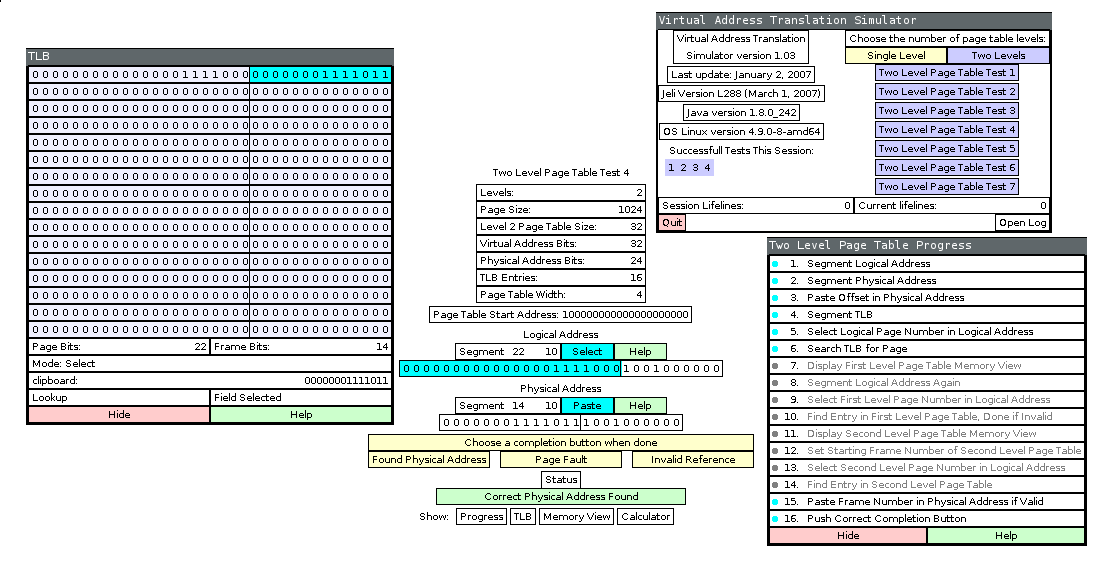
\includegraphics[width=\textwidth]{address.png}
\end{figure}

\end{document}

